\documentclass[hidelinks]{ctexart}

\usepackage{van-de-la-illinoise}
\usepackage{cmbright}
\usepackage{nccmath}
\usepackage[paperheight=297mm,paperwidth=240mm,top=.2in,left=.1in,right=.1in,bottom=.2in, landscape]{geometry}
\usepackage{tensor}

\definecolor{graybg}{RGB}{228,235,243}
\definecolor{titlepurple}{RGB}{150,131,104}
\definecolor{shadegray}{RGB}{102,119,136}
\definecolor{itemgray}{RGB}{163,149,128}
\definecolor{mathnormalblack}{RGB}{0,0,0}
\pagecolor{graybg}

\setCJKmainfont{STHeitiSC-Light}
\setmainfont{Arial}

\usepackage{multicol}
\setlength{\columnsep}{.1in}

\newcommand{\raisedrule}[2][0em]{\qquad}
%\leaders\hbox{\rule[#1]{1pt}{#2}}\hfill}
\newcommand{\wdiv}{\,·\,}

\setlength{\parindent}{0pt}

\setCJKfamilyfont{pfsc}{STYuanti-SC-Regular}
\newcommand{\titlefont}{\CJKfamily{ttt}}
\setCJKfamilyfont{ttt}{STFangsong}
\newcommand{\mathtextfont}{\CJKfamily{ttt}}
\def\bili#1#2{#2}

\newdimen\indexlen
\def\newheader#1{%
\def\probindex{#1}
\setlength\indexlen{\widthof{\Large\color{titlepurple} #1\qquad}}
\vspace{1em}
{\Large\color{titlepurple} #1\qquad}
\raisebox{.5em}{\tikz \fill[titlepurple,opacity=.2,path fading=east] (0,0.05em) rectangle (\dimexpr\linewidth-\indexlen\relax,0em);}
}
\def\mathitem#1{\text{\color{itemgray}#1}}
\def\mathcomment#1{\text{\color{lightgray}\quad \texttt{\#}\kern-0pt#1}}
\def\mathheadcomment#1{\text{\color{lightgray}\texttt{\#}\kern-0pt#1}}
\def\midbreak{\smash{\raisebox{1.5em}{\smash{\tikz \path[opacity=.2,left color=white,right color=white,middle color=black] (0,0.05em) rectangle (\linewidth,0em);}}}
\vspace{-4em}}
\newtcolorbox{cheatresume}{enhanced, arc=.5pt, left=.5em, frame hidden, boxrule=0pt, colback=white, fuzzy halo=.05pt with lightgray, shadow={.4pt}{-.4pt}{0pt}{fill=shadegray,opacity=0.3}}

\usetikzlibrary{arrows.meta}

\begin{document}

\begin{multicols*}{3}[\centerline{\titlefont 原子の波動関数及び微細構造、Zeeman効果など}]
\raggedcolumns%
\newheader{\bili{}{水素原子ノ波動関数}}
\begin{cheatresume}
    \begin{flalign*}
        & \mathitem{動径方向} && R_{nl}\pare{r} \propto e^{-\rho/2}\rho^l L_{n+1}^{2l+1}\pare{\rho},\quad \rho = \sqrt{-\frac{8mE}{\hbar^2}}r && \\
        & && R_{10}\pare{r} = 2\pare{\frac{Z}{a_0}}^{3/2}e^{-Ze/a_0} && \\
        & \mathitem{波動関数} && u = R_{nl}\pare{r}Y_{lm}\pare{\theta,\varphi} && \\
        & && n \ge 1,\quad l = 0,\cdots, n - 1, \quad m = -l,\cdots,+l &&
    \end{flalign*}
\end{cheatresume}
\newheader{\bili{}{水素原子ノ微細構造}}
\begin{cheatresume}
    \begin{flalign*}
        %& \mathitem{選択率} && \Delta n = \forall,\quad \Delta l = \pm 1,\quad \Delta m = 0, \pm 1 && \\
        & \mathitem{Bohr磁子} && \mu\+_B_ = \frac{e\hbar}{2m_e} && \\
        & \mathitem{軌道磁気} && \+v\mu_l = -\mu\+_B_ \frac{\+vL}{\hbar},\quad \mu_{lz} = -m_l\mu\+_B_ && \\
        & \mathitem{スピン磁気} && \+v\mu_s = -g_s \mu\+_B_ \frac{\+vS}{\hbar},\quad \mu_{sz} = -g_sm_s\mu\+_B_ &&
    \end{flalign*}
    \midbreak
    \begin{flalign*}
        & \begin{array}{@{}l}
            \mathitem{スピン軌道項} \\
            \color{lightgray}E_n<0 \\
            \color{lightgray}l\neq 0 \text{と} \\
        \end{array} &&  \begin{array}{ll}
            \displaystyle -E_n \frac{\alpha^2 Z^2}{n^2} \frac{n}{\displaystyle \pare{2l+1}\pare{l+1}}, & {\displaystyle j = l + \half} \\
            \displaystyle +E_n \frac{\alpha^2 Z^2}{n^2} \frac{n}{\displaystyle l\pare{2l+1}}, & {\displaystyle j = l - \half}
        \end{array} && \\
        & \mathitem{運動エネルギー} && -E_n\frac{\alpha^2Z^2}{n^2}\pare{\frac{3}{4} - \frac{n}{\displaystyle l+1/2}} && \\
        & \mathitem{Darwin}\mathcomment{l=0} && -E_n \frac{\alpha^2Z^2}{n} && \\
        & \mathitem{全補正} && -E_n \frac{\alpha^2Z^2}{n^2}\pare{\frac{3}{4} - \frac{n}{j+1/2}} &&
    \end{flalign*}
    \midbreak
    \begin{flalign*}
        & \mathitem{超微細構造} && \Delta E = \frac{a}{2}\brac{F\pare{F+1} - J\pare{J+1} - I\pare{I+1}} %\mathcomment{水素の$\displaystyle I=\half$}
        && \\
        & \mathheadcomment{水素様と} && a = -2g_I\pare{\frac{m_e}{M_p}}\frac{\alpha^2 Z}{n}E_n \rec{j\pare{j+1}\pare{2l+1}} &&
    \end{flalign*}
    \midbreak
    \vspace{3.5cm}
    \begin{center}
        \smash{\begin{tikzpicture}[yscale=0.7,xscale=0.9]
        \draw[densely dotted,draw=lightgray] (6,-1.5) -- (8.5,-1.5);
        \draw[densely dotted,draw=lightgray]
            (1,0) -- (1.5,-1.5)
            (1,0) -- (1.5,-0.5) -- (3,-0.5)
            (1,4) -- (1.5,3.5) -- (4.5,3.5)
            (1,4) -- (1.5,2.5) -- (3,2.5)
            (1,4) -- (1.5,1.5)
        ;
        \draw[-latex,draw=lightgray] (1.75,1.5) -- (3.25,-1.5);
        \draw[-latex,draw=lightgray] (2.25,1.5) -- (3.25,-0.5);
        \draw[-latex,draw=lightgray] (4.75,2.5) -- (3.75,-0.5);
        \draw[-latex,draw=lightgray] (5.25,2.5) -- (3.75,-1.5);
        \draw[-latex,draw=lightgray] (5,3.5) -- (3.5,-0.5);
        \draw[-latex,draw=lightgray] (3.5,2.5) -- (1.75,-1.5);
        \draw[-latex,draw=lightgray] (3.5,1.5) -- (2.25,-1.5);
        \draw
            (0,0) -- (1,0) node[midway,above=-.2em] {$\scriptstyle n=2$}
            (0,4) -- (1,4) node[midway,above=-.2em] {$\scriptstyle n=3$}
            (1.5,-1.5) -- (2.5,-1.5) node[midway,above=-.3em] {$\scriptstyle 2{^2\mathrm S}_{1/2}$}
            (3,-1.5) -- (4,-1.5) node[midway,above=-.3em] {$\scriptstyle 2{^2\mathrm P}_{1/2}$}
            (3,-0.5) -- (4,-0.5) node[midway,above=-.3em] {$\scriptstyle 2{^2\mathrm P}_{3/2}$}
            %
            (1.5,1.5) -- (2.5,1.5) node[midway,above=-.3em] {$\scriptstyle 3{^2\mathrm S}_{1/2}$}
            (3,1.5) -- (4,1.5) node[midway,above=-.3em] {$\scriptstyle 3{^2\mathrm P}_{1/2}$}
            (3,2.5) -- (4,2.5) node[midway,above=-.3em] {$\scriptstyle 3{^2\mathrm P}_{3/2}$}
            (4.5,2.5) -- (5.5,2.5) node[midway,above=-.3em] {$\scriptstyle 3{^2\mathrm D}_{3/2}$}
            (4.5,3.5) -- (5.5,3.5) node[midway,above=-.3em] {$\scriptstyle 3{^2\mathrm D}_{5/2}$}
            ;
        \draw[-latex] (4.5,-1) -- (5.5,-1) node[midway,above=-.1em] {\color{lightgray}\scriptsize Lamb};
        \draw
            (6,-1.1) -- (7,-1.1) node[midway,above=-.3em] {$\scriptstyle 2{^2\mathrm S}_{1/2}$}
            (7.5,-1.65) -- (8.5,-1.65) node[midway,above=-.3em] {$\scriptstyle 2{^2\mathrm P}_{1/2}$}
            (7.5,-0.5) -- (8.5,-0.5) node[midway,above=-.3em] {$\scriptstyle 2{^2\mathrm P}_{3/2}$};
        \draw[line width=.01pt,latex-latex,draw=lightgray] (7.25,-1.65) -- (7.25,-1.1);
        \draw[-latex] (6.5,-0.3) -- (7,2.5) node[midway,above=-.1em,sloped] {\color{lightgray}\scriptsize 超微細};
        \draw
        (7.5,2.5) -- (8.5,2.5) node[midway,above=-.3em] {$\scriptstyle 2{^2\mathrm S}_{1/2}$}
        (9,1.9) -- (10,1.9) node[midway,above=-.2em] {$\scriptstyle F=0$}
        (9,2.7) -- (10,2.7) node[midway,above=-.2em] {$\scriptstyle F=1$}
        ;
        \draw[densely dotted,draw=lightgray]
        (8.5,2.5) -- (9,1.9)
        (8.5,2.5) -- (9,2.7)
        ;
    \end{tikzpicture}}
    \end{center}
\end{cheatresume}
\columnbreak
\newheader{\bili{}{アルカリ金属}}
\begin{cheatresume}
    \begin{flalign*}
        & \mathitem{エネルギー} && E_{nl} = -\half \mu\alpha^2c^2 \rec{\pare{n-\Delta_{nl}}^2} && \\
        & \mathitem{微細構造} && \delta E_{ls} = %\begin{cases}
            %0, & l=0 \\
            \displaystyle \frac{\mu c^2\alpha^4 Z^{*4}_{fs}}{2n^{*3}} \rec{l\pare{l+1}}, \quad l>0
        %\end{cases}
        && 
    \end{flalign*}
\end{cheatresume}
\newheader{\bili{}{磁場中においた}}
\begin{cheatresume}
    \begin{flalign*}
        & \+:c5l{\mathitem{弱い磁場の場合(Zeeman効果)}\hfill \mathcomment{$B\ll Z^4\SI{}{\tesla}$\quad}} \\
        & \mathitem{磁気} && \+v\mu_j = -g_j\mu\+_B_\frac{\+vJ}{\hbar},\quad g_j = \frac{3}{2} + \frac{s\pare{s+1} - l\pare{l+1}}{2j\pare{j+1}} && \\
        & \mathitem{シフト} && E' = E + m_j g_j \mu\+_B_B && \\
        & \mathitem{波数} && \tilde{\nu} = \tilde{\nu}_0 + \+sL\pare{m_2g_2 - m_1g_1}\mathcomment{$m_2\mapsto m_1$} && \\
        & && \+sL = \frac{\mu\+_B_B}{hc} = \SI{0.466}{\per\centi\meter}\cdot B\SI{}{\per\tesla} &&
    \end{flalign*}
    \vspace{2.4cm}
    \begin{center}
        \smash{\begin{tikzpicture}[yscale=0.45]
            \draw (0,0) -- (1,0) node[midway,above=-.2em] {$\scriptstyle 3\mathrm{s}$}
            (1.5,0) -- (2.5,0) node[midway,above=-.3em] {$\scriptstyle 3{^2\mathrm S}_{1/2}$}
            (0,3) -- (1,3) node[midway,above=-.2em] {$\scriptstyle 3\mathrm{p}$}
            (1.5,2) -- (2.5,2) node[midway,above=-.3em] {$\scriptstyle 3{^2\mathrm P}_{1/2}$}
            (1.5,4) -- (2.5,4) node[midway,above=-.3em] {$\scriptstyle 3{^2\mathrm P}_{3/2}$}
            (3,5.2) -- (5,5.2) node[right] (p32mmg) {$\scriptstyle +3/2,+2$}
            (3,4.4) -- (5,4.4) node[right] {$\scriptstyle +1/2,+2/3$}
            (3,3.6) -- (5,3.6) node[right] {$\scriptstyle -1/2,-2/3$}
            (3,2.8) -- (5,2.8) node[right] {$\scriptstyle -3/2,-2$}
            (3,2.2) -- (5,2.2) node[right] {$\scriptstyle +1/2,+1/3$}
            (3,1.8) -- (5,1.8) node[right] {$\scriptstyle -1/2,-1/3$}
            (3,0.6) -- (5,0.6) node[right] {$\scriptstyle +1/2,+1$}
            (3,-0.6) -- (5,-0.6) node[right] {$\scriptstyle -1/2,-1$}
            (p32mmg) node[above=.5em] {$\scriptstyle m\quad mg$}
            ;
            \draw[-latex,draw=lightgray] (3.1,1.8) -- (3.1,0.6);
            \draw[-latex,draw=lightgray] (3.3,2.2) -- (3.3,0.6);
            \draw[-latex,draw=lightgray] (3.5,1.8) -- (3.5,-0.6);
            \draw[-latex,draw=lightgray] (3.7,2.2) -- (3.7,-0.6);
            \draw[-latex,draw=lightgray] (3.9,3.6) -- (3.9,0.6);
            \draw[-latex,draw=lightgray] (4.1,2.8) -- (4.1,-0.6);
            \draw[-latex,draw=lightgray] (4.3,4.4) -- (4.3,0.6);
            \draw[-latex,draw=lightgray] (4.5,3.6) -- (4.5,-0.6);
            \draw[-latex,draw=lightgray] (4.7,5.2) -- (4.7,0.6);
            \draw[-latex,draw=lightgray] (4.9,4.4) -- (4.9,-0.6);
            \draw[densely dotted,draw=lightgray]
            (1,3) -- (1.5,4)
            (1,3) -- (1.5,2)
            (1,0) -- (1.5,0)
            (2.5,0) -- (3,0.6)
            (2.5,0) -- (3,-0.6)
            (2.5,2) -- (3,1.8)
            (2.5,2) -- (3,2.2)
            (2.5,4) -- (3,2.8)
            (2.5,4) -- (3,3.6)
            (2.5,4) -- (3,4.4)
            (2.5,4) -- (3,5.2)
            ;
            \draw (2,-0.7) node[below] {\scriptsize\color{lightgray}\begin{tabular}{cc}
                スピン軌道項\\ $j$による
            \end{tabular}}
            ;
            \draw (4,-0.7) node[below] {\scriptsize\color{lightgray}\begin{tabular}{cc}
                Zeeman効果\\ $m_j$による
            \end{tabular}}
            ;
        \end{tikzpicture}}
    \end{center}
    \midbreak
    \begin{flalign*}
        & \+:c5l{\mathitem{強い磁場の場合(Paschen-Back効果)}\hfill \mathcomment{$B> Z^4\SI{}{\tesla}$\quad}} \\
        & \mathitem{シフト} && E' = E + \pare{m_l + 2m_s}\mu\+_B_B && \\
        & \mathitem{波数} && \tilde{\nu} = \tilde{\nu}_0 + \frac{\mu\+_B_B}{hc}\pare{m_{l2}-m_{l1}} \mathcomment{$m_{l2}\mapsto m_{l1}$} && \\
        & \mathitem{スピン軌道項} && E'' = E' + \xi_{nl}m_lm_s &&
    \end{flalign*}
    \vspace{2.0cm}
    \begin{center}
        \smash{\begin{tikzpicture}[yscale=0.5]
            \draw[densely dotted,draw=lightgray]
            (2.5,4) -- (5,4) -- (7,4)
            (2.5,3.5) -- (5,3.5) -- (7,3.5)
            (2.5,3) -- (5,3) -- (7,3)
            (2.5,2.5) -- (5,2.5) -- (7,2.5)
            (2.5,2) -- (5,2) -- (7,2)
            (2.5,0.8) -- (5,0.8) -- (7,0.8)
            (2.5,-0.2) -- (5,-0.2) -- (7,-0.2)
            ;
            \draw (0,0.3) -- (1,0.3) node[midway,above=-.2em] {$\scriptstyle 3\mathrm{s}$}
            (0,3) -- (1,3) node[midway,above=-.2em] {$\scriptstyle 3\mathrm{p}$}
            (1.5,0.8) -- (2.5,0.8) node[right] {$\scriptstyle \phantom{+}0,+1/2,\phantom{2}+\mu\+_B_B$}
            (1.5,-0.2) -- (2.5,-0.2) node[right] {$\scriptstyle \phantom{+}0,-1/2,\phantom{2}+\mu\+_B_B$}
            (1.5,2.0) -- (2.5,2.0) node[right] {$\scriptstyle -1,-1/2,-2\mu\+_B_B$}
            (1.5,2.5) -- (2.5,2.5) node[right] {$\scriptstyle \phantom{+}0,-1/2,\phantom{2}-\mu\+_B_B$}
            (1.5,3) -- (2.5,3) node[right] {$\scriptstyle \pm 1,\mp 1/2,\phantom{+\mu\+_B_B}0$}
            (1.5,3.5) -- (2.5,3.5) node[right] {$\scriptstyle \phantom{+}0,+1/2,\phantom{2}+\mu\+_B_B$}
            (1.5,4) -- (2.5,4) node[right](3ptop) {$\scriptstyle +1,+1/2,+2\mu\+_B_B$}
            (3ptop) node[above=.3em] {$\scriptstyle m_l\enspace m_s\enspace \Delta E$}
            (5,4.15) -- (7,4.15) node[right](sltop) {$\scriptstyle \xi_{3\mathrm p}/2$}
            (5,3.5) -- (7,3.5) node[right] {$\scriptstyle 0$}
            (5,2.85) -- (7,2.85) node[right] {$\scriptstyle -\xi_{3\mathrm p}/2$}
            (5,2.5) -- (7,2.5) node[right] {$\scriptstyle 0$}
            (5,2.15) -- (7,2.15) node[right] {$\scriptstyle \xi_{3\mathrm p}/2$}
            (5,0.8) -- (7,0.8) node[right] {$\scriptstyle 0$}
            (5,-0.2) -- (7,-0.2) node[right] {$\scriptstyle 0$}
            (sltop) node[above=.3em] {$\scriptstyle \Delta E'$}
            ;
            \draw[-latex,draw=lightgray] (5.1,2.15) -- (5.1,-0.2);
            \draw[-latex,draw=lightgray] (5.4,2.85) -- (5.4,0.8);
            \draw[-latex,draw=lightgray] (5.85,2.5) -- (5.85,-0.2);
            \draw[-latex,draw=lightgray] (6.15,3.5) -- (6.15,0.8);
            \draw[-latex,draw=lightgray] (6.6,2.85) -- (6.6,-0.2);
            \draw[-latex,draw=lightgray] (6.9,4.15) -- (6.9,0.8);
            \draw[densely dotted,draw=lightgray]
            (1,0.3) -- (1.5,0.8)
            (1,0.3) -- (1.5,-0.2)
            (1,3) -- (1.5,2)
            (1,3) -- (1.5,2.5)
            (1,3) -- (1.5,3)
            (1,3) -- (1.5,3.5)
            (1,3) -- (1.5,4)
            ;
            \draw (2,-0.3) node[below] {\scriptsize\color{lightgray}\begin{tabular}{cc}
                Paschen-Back効果\\ $m_l+2m_s$による
            \end{tabular}}
            ;
            \draw (6,-0.3) node[below] {\scriptsize\color{lightgray}\begin{tabular}{cc}
                スピン軌道項\\ $m_lm_s$による
            \end{tabular}}
            ;
        \end{tikzpicture}}
    \end{center}
    \midbreak
    \tikzset{
    partial ellipse/.style args={#1:#2:#3}{
        insert path={+ (#1:#3) arc (#1:#2:#3)}
    }}
    \begin{flalign*}
        & \mathitem{偏光} && m\downarrow_{-1}\raisebox{-.4em}{\smash{\begin{tikzpicture}
    \draw (0,0) ellipse (.8em and .3em);
    \draw[draw=gray,-latex] (0,-.3) -- (0,+.3);
    \draw[draw=gray,-latex] (-.2,0) -- (+.8,0);
    \draw[latex-latex] (.3,-.15) -- (.7,.15);
    \draw[-latex] (0,0) [partial ellipse=210:330:.8em and .3em];
\end{tikzpicture}}}\enspace {\color{lightgray}\vert}\Delta m = 0\enspace\raisebox{-.5em}{\smash{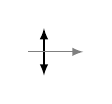
\begin{tikzpicture}
    \draw[latex-latex] (0,-.3) -- (0,+.3);
    \draw[draw=gray,-latex] (-.2,0) -- (+.5,0);
\end{tikzpicture}}}{\color{lightgray}\vert}\enspace m\uparrow^{+1}\raisebox{-.4em}{\smash{\begin{tikzpicture}
    \draw (0,0) ellipse (.8em and .3em);
    \draw[draw=gray,-latex] (0,-.3) -- (0,+.3);
    \draw[draw=gray,-latex] (-.2,0) -- (+.8,0);
    \draw[latex-latex] (.3,-.15) -- (.7,.15);
    \draw[-latex] (0,0) [partial ellipse=330:210:.8em and .3em];
\end{tikzpicture}}} &&
    \end{flalign*}
\end{cheatresume}
\columnbreak
\newheader{\bili{}{二原子分子}}
\begin{cheatresume}
    \begin{flalign*}
        & \mathitem{未然}
    \end{flalign*}
\end{cheatresume}

\end{multicols*}

\end{document}
